\documentclass{article}

\usepackage{mathpazo}

% -- PACKAGES -----------------------------------------------------------

\usepackage{times}
\usepackage{graphicx}
\usepackage{verbatim}
\usepackage{amsmath, amssymb}
\usepackage{booktabs}

% TODO have a look:
%\usepackage{subfigure}

\usepackage{color}
\usepackage{url}
\usepackage{a4wide, booktabs}
\usepackage[a4paper,top=2.5cm,bottom=3.0cm,left=2cm,right=2cm,%
            bindingoffset=5mm]{geometry}
\usepackage[bookmarks,
            colorlinks=true,
            linkcolor=blue,
            pdfauthor={Andrea Zito, Giovanni Simoni},
            pdftitle={Report 1: Interference between Bluetooth and 802.11
                      Wireless}]{hyperref}
\usepackage{multicol}
%\newenvironment{multicols}[1]{}{}

% -- COMMANDS -----------------------------------------------------------

\newcommand{\batman}{{\textsf BATMAN}}
\newcommand{\olsr}{{\textsf OLSR}}

\newcommand{\station}[1]{{\textsf Station #1}}
\newcommand{\primitive}[1]{{\footnotesize \tt #1()}}
\newcommand{\library}[1]{{\textsf #1}}

\newcommand{\Variable}[1]{\mbox{\emph{#1}}}

% Units of measurement:
\newcommand{\Sec}{s}
\newcommand{\uSec}{\mu\Sec}
\newcommand{\MHz}{MHz}
\newcommand{\GHz}{GHz}
\newcommand{\Slot}{\Variable{slot}}
\newcommand{\Frame}{\Variable{frame}}
\newcommand{\FrameSlot}{\Frame/\Slot}

\newcommand{\Bit}{\mbox{\footnotesize bit}}
\newcommand{\Byte}{\mbox{\footnotesize byte}}

\newcommand{\MBit}{M\Bit}
\newcommand{\MByte}{M\Byte}

\newcommand{\MBitSec}{\MBit/\Sec}
\newcommand{\MByteSec}

\newcommand{\KByteSec}{k\Byte/\Sec}
\newcommand{\KBitSec}{k\Bit/\Sec}

% Probability
\newcommand{\RandomDist}{\sim}
\newcommand{\Probability}[1]{\mbox{{\sf P}}\left(#1\right)}
\newcommand{\Average}[1]{\mathbb{E}\left[#1\right]}
\newcommand{\Variance}[1]{\mathbb{V}\left[#1\right]}
\newcommand{\Normal}[2]{\mathcal{N}\left(#1, #2\right)}
\newcommand{\Interval}[2]{\left[#1, #2\right]}

% Other stuff
\newcommand{\HRule}{\rule{\linewidth}{0.1mm}}
\newcommand{\Ceiling}[1]{\left\lfloor#1\right\rfloor}



\begin{document}
  \begin{titlepage}
    \centering

     \begin{figure}[ht]
       \centering
       
\includegraphics[angle=-90, keepaspectratio=true, width=8cm]
                       {images/logo}
     \end{figure}

     { \large \bfseries Nomadic Comunication\par AA 2009-2010 }\par

     \vspace{1.5cm}
     { \Large \bfseries \textcolor{blue}
        {Report 2: Mesh Networks}
        \par }
     \vspace{1.0cm}
     { \large \bfseries {Group N. ?} \par }
     \vspace{0.3cm}

     {\large \bfseries {Andrea Zito, Giovanni Simoni}}

     \vspace{1.0cm}

\begin{abstract}

    In this report we are going to analyze and compare the behaviour of
    \batman\cite{bib:BATMAN} and \olsr\cite{bib:OLSR}, two softwares each
    of which implement a \emph{proactive meshed networks} routing
    protocol.

\end{abstract}

\end{titlepage}

\thispagestyle{empty}
\tableofcontents

\clearpage
\setcounter{page}{1}

\section{Introduction} \label{sec:Intro}
\vspace{-3mm}\HRule

    \begin{multicols}{2}
    An interesting issue about \emph{meshed networks} is how they influence
the network performances with respect to configurations in which routes are
defined statically. The comparison we worked on takes in account
\batman\cite{bib:BATMAN} and \olsr\cite{bib:OLSR}, both implementing mesh
routing protocols.

\subsection{About \batman}

    The \batman\ protocol is based on a proactive approach exploiting a
    flooding technique. Each host in a \batman\ mesh network produces, on a
    regular basis, an \emph{Originator Message} which is sent in
    broadcast and gets received by all directly reachable neighbors. Every
    \emph{Originator Message} contains, among other things, a
    \emph{Sequence Number} and a \emph{TTL}.

    Each node keeps, for any destination host, a sliding window of
    recent sequence numbers. The window gets moved as new sequence numbers
    arrive, and this makes oldest sequence numbers obsolete. The preferred
    route is given by the host having the maximum number of entries in the
    sliding window.  So far, each packet contains only a few data, and
    doesn't give any kind of information on how the routing table is
    structured in the sender Originator.

    The node is in charge of re-broadcasting a message from another node
    if:
    \begin{itemize}
    \item   The Sequence Number hasn't been seen yet;
    \item   The message's TTL hasn't been expired.
    \end{itemize}

    The suggested period for the flooding operation is of 1 second, thus
    in an environment configured with default values this is the actual
    frequency of the flooding operation.

\subsection{About \olsr}

    The protocol is far more complex than \batman, as it's best suited for
    extended and complex networks. Such complexity boils down to
    each host periodically sending of a part of the \emph{link-state}
    table. The details are beyond the purposes of this report, since
    they're not affecting that much the actual network interaction. What
    really concerns us is the software timing:
    \begin{itemize}
    \item   A probing for the direct neighbors is achieved by means of a
            periodically broadcasted \emph{Hello} message. The
            \Const{HELLO\_INTERVAL} constant, determining the broadcasting
            period, is of 2 seconds;
    \item   Some of the direct neighbors are used as relay nodes, and are
            targeted with messages of type \emph{Topology Control}.
            The \Const{TC\_INTERVAL} constant schedules a direct
            communication every 5 seconds.
    \end{itemize}

\subsection{Experiments with meshed networks}

    The comparison has been achieved by means of two different classes
    of tests: the first one aims to measure the worsening of the network
    performance due to the two protocols, the second one tests how
    responsive are the protocols with respect to changes in the
    network topology.

    The needed data has been retrieved by using some tools:
    \begin{itemize}
    \item   Data about latency has been obtained by means of the
            \emph{ping} tool;
    \item   Throughput has been measured with
            \netperf\cite{bib:NetPerf};
    \item   Statistics about protocol responsiveness for \batman\ and
            \olsr\ have been extrapolated by parsing the output of the
            two softwares respectively.
    \end{itemize}

\subsection{The testbed}

    The testbed has been composed by four laptops equipped with
    \emph{Ubuntu 10.10 GNU/Linux} operating systems. We used the following
    softwares:
    \begin{description}
    \item[\netperf] Version \emph{2.4.4-5ubuntu2};
    \item[\batman] Daemon version \emph{0.3.2-5} (userspace version);
    \item[\olsr] Daemon version \emph{0.5.6-r7-1};
    \item[iptables] Version \emph{1.4.4-2ubuntu3};
    \item[wireshark] Version \emph{1.2.11-4build0.10.10.10}.
    \end{description}

    Depending on the tests, the network topologies have been arranged
    specifically, so far each section of this report will be provided with
    a paragraph describing it.


    \end{multicols}

\section{Impact on throughput} \label{sec:ImpactThroughput}
\vspace{-3mm}\HRule

    \begin{multicols}{2}
    \subsection{Test introduction}

    The throughput is probably the most relevant index of the network
    quality. In the context of \emph{mesh networking} a natural concern is
    how the overhead coming from the underlaying routing protocol affects
    it.

    As we previously mentioned, both the protocols we worked
    with are of the \emph{pro-active} family: they periodically sends
    packets which are used to build and maintain the topology. Obviously
    the number of control packets generated by the routing protocol grows
    with the number of nodes which are part of the network thus, since our
    testbed was composed by just a few hosts, what we reasonably expected
    was a minimal impact on the overall performances.

    The core of the experiment consisted in a simple throughput test with
    \netperf\ on three different network topologies. For both the
    analyzed mesh protocols we performed the test while the protocol's
    software was running. We also run an instance of the test with
    statically compiled routes in order to obtain an \emph{ideal overhead
    situation} to be used as term of comparison.

    For each combination of network topology and routing protocol, we
    executed 10 consecutive \netperf\ measurement, each one delayed by 10 seconds
    from the previous. Each run lasted 60 seconds and was performed by
    running the following command on the \emph{source} machine (10.0.0.65):
\begin{verbatim}
netperf -H 10.0.0.67 -D 1 -l 60
\end{verbatim}

    In order to keep coherence between tests, we always used the host
    10.0.0.67 as target.

    \subsubsection{Topology}

        The \emph{direct link} topology is the simplest. Only two laptops
        have been enabled (see Figure~\ref{pic:LayoutDirect}):
        \begin{itemize}
        \item   The \emph{Source} node (address 10.0.0.65);
        \item   The \emph{Sink} node (address 10.0.0.67).
        \end{itemize}

        \Picture{images/direct}
                {.49\columnwidth}
                {Configuration with single direct link}
                {pic:LayoutDirect}

    \subsubsection{Results}

        In this situation the message exchange is very limited: every
        synchronization step consists in the two hosts simply exchanging a
        few UDP packets (as described in Section~\ref{sec:Intro}). The
        network performances measure
        confirms our hypothesis: as shown in Table~\ref{tab:ThrDirect} the
        performance variation is so minimal that is more likely to be
        caused by the different condition of the wireless channel
        among experiments, rather then the actual overhead of the
        protocols.

        \Picture{images/throughput_plot_direct}
                {0.7 \columnwidth}
                {Impact of the meshing protocols on the throughput of the
                 direct link topology. The three boxplots show,
                 respectively, the performance with \emph{static routes},
                 \batman\ and \olsr.}
                {pic:ThpDirect}

        \begin{table}[htbp]
            \centering
            \begin{tabular}{rcccccccc}
            \toprule
            Protocol & Average & Variance & Min & 1st Quartile &
            Median & 3rd Quartile & Max & Comp. w.r.t.\\
            & \footnotesize{\MBitsSec} &
            & \footnotesize{\MBitsSec} &
              \footnotesize{\MBitsSec} &
              \footnotesize{\MBitsSec} &
              \footnotesize{\MBitsSec} &
              \footnotesize{\MBitsSec} & Static\\

            \midrule
            Static      & 16.970 & 0.191 & 15.74 & 16.67 & 16.97 & 17.26
                        & 18.08  & - \\
            \batman\    & 16.926 & 0.251 & 15.41 & 16.58 & 16.94 & 17.3
                        & 18.4   & 0.997 \\
            \olsr\      & 16.990 & 0.313 & 14.98 & 16.65 & 17.02 & 17.35
                        & 18.86  & 1.001 \\
            \bottomrule
            \end{tabular}
            \caption{Throughput result for direct topology. The last
                     column shows a proportional comparison with the
                     average throughput of the statically compiled
                     routes.}
            \label{tab:ThrDirect}
        \end{table}

\subsection{Test with 1 hop}

    \subsubsection{Topology}

        The \emph{1 hop} topology is composed by 3 computer arranged
        in a chain (see Figure~\ref{pic:Layout1Hop}):
        \begin{itemize}
        \item   The \emph{Source} node (address 10.0.0.65);
        \item   The node acting as bridge (address 10.0.0.66);
        \item   The \emph{Sink} node (address 10.0.0.67).
        \end{itemize}

        \Picture{images/1hop}
                {.90\columnwidth}
                {Configuration with 1 hop}
                {pic:Layout1Hop}

        To implement this scheme we needed to prevent the \emph{Source}
        node from communicating directly with the \emph{Sink} one and vice
        versa, but since we were operating with a wireless medium it
        wasn't possible to physically stop the 2 computer from seeing each
        other. As workaround we exploited \emph{iptables} to filter out
        incoming packet based on the MAC address of the sender.

        \begin{itemize}
        \item On \emph{Source}:
            \begin{verbatim}
iptables -A INPUT -m mac --mac-source $(sinkMAC) -j DROP;
            \end{verbatim}

        \item On \emph{sink}:
            \begin{verbatim}
iptables -A INPUT -m mac --mac-source $(sourceMAC) -j DROP;
            \end{verbatim}

        \end{itemize}

    \subsubsection{Results}

        As before it was reasonable to assume the overhead imposed by
        the routing protocols to be negligible, as the number of node was
        really small: again we expected to measure equivalent average
        throughputs. Instead the results we obtained show otherwise.
        As we can clearly see in  Figure~\ref{pic:Thp1Hop} and
        Table~\ref{tab:Thr1Hop}, when using \batman\ and \olsr\, the average
        throughput decreases significantly while the variance increases notably.

        In our opinion this result does not provide a truthful
        picture of the reality. This consideration is sustained by
        the fact that we have more overhead than in a 2 hops configuration
        (see Paragraph~\ref{subsec:2hop}), in which intuitively the
        interference should be much more detectable. At any rate, we report
        the obtained experimental data.

        \Picture{images/throughput_plot_1hop}
                {0.7 \columnwidth}
                {Impact of the meshing protocols on the throughput of the
                 1-hop topology. The three boxplots show, respectively, the
                 performance with \emph{static routes}, \emph{\batman} and
                 \emph{\olsr}}
                {pic:Thp1Hop}

        \begin{table}[htbp]
            \centering
            \begin{tabular}{rcccccccc}
            \toprule
            Route & Average & Variance & Min & 1st Quartile &
            Median & 3rd Quartile & Max & Comp. w.r.t.\\
            & \footnotesize{\MBitsSec} & & \footnotesize{\MBitsSec} & \footnotesize{\MBitsSec} &
            \footnotesize{\MBitsSec} & \footnotesize{\MBitsSec} & \footnotesize{\MBitsSec} & Static\\
            \midrule
            Static      & 8.496 & 1.118 & 2.635 & 8.09 & 8.62 & 9.08
                        & 11.12 & - \\
            \batman\    & 7.973 & 2.197 & 1.455 & 7.425 & 8.27 & 8.855
                        & 11.71 & 0.938 \\
            \olsr\      & 6.924 & 7.68 & 0.096 & 6.91 & 8.01 & 8.62
                        & 10.21 & 0.815 \\
            \bottomrule
            \end{tabular}
            \caption{Throughput result for 1hop topology. The last
                     column shows a proportional comparison with the
                     average throughput of the statically compiled
                     routes.}
            \label{tab:Thr1Hop}
        \end{table}

\subsection{Test with 2 hop} \label{subsec:2hop}

    \subsubsection{Topology}

        The \emph{2 hops} topology is composed by 4 computers disposed
        in a chain (see Figure~\ref{pic:Layout2Hop}):
        \begin{itemize}
        \item   The \emph{Source} node (address 10.0.0.65);
        \item   The node acting as first hop (address 10.0.0.66);
        \item   The node acting as second hop (address 10.0.0.68);
        \item   The \emph{Sink} node (address 10.0.0.67).
        \end{itemize}

        \Picture{images/2hop}
                {.90\columnwidth}
                {Configuration with 2 hop}
                {pic:Layout2Hop}

        \noindent The rules for \emph{iptables} we used to implement this
        configuration are the following:

        \begin{itemize}
        \item On the \emph{Source} node:
        \begin{verbatim}
iptables -A INPUT -m mac --mac-source $(sinkMAC) -j DROP;
iptables -A INPUT -m mac --mac-source $(hop2MAC) -j DROP;
        \end{verbatim}

        \item On the first hop:
        \begin{verbatim}
iptables -A INPUT -m mac --mac-source $(sinkMAC) -j DROP;
        \end{verbatim}

        \item On the second hop:
        \begin{verbatim}
iptables -A INPUT -m mac --mac-source $(sourceMAC) -j DROP;
        \end{verbatim}

        \item On the \emph{Sink}
        \begin{verbatim}
iptables -A INPUT -m mac --mac-source $(sourceMAC) -j DROP;
iptables -A INPUT -m mac --mac-source $(hop1MAC) -j DROP;
        \end{verbatim}

        \end{itemize}

    \subsubsection{Results}

        This time the results are more compatible with our hypothesis.
        As in the direct link topology the throughput difference between
        the three measurements is negligible and most likely caused by
        noise on the wireless channel.

        \Picture{images/throughput_plot_2hop}
                {0.7 \columnwidth}
                {Impact of the meshing protocols on the throughput of the
                 2-hops topology. The three boxplots show, respectively,
                 the performance with \emph{static routes}, \emph{\batman}
                 and \emph{\olsr}}
                {pic:Thp2Hops}

        \begin{table}[htbp]
            \centering
            \begin{tabular}{rcccccccc}
            \toprule
            Route & Average & Variance & Min & 1st Quartile &
            Median & 3rd Quartile & Max & Comp. w.r.t.\\
            & \footnotesize{\MBitsSec} & & \footnotesize{\MBitsSec} & \footnotesize{\MBitsSec} &
            \footnotesize{\MBitsSec} & \footnotesize{\MBitsSec} & \footnotesize{\MBitsSec} & Static\\
            \midrule
            Static      & 5.344 & 2.183 & 1.332 & 4.82 & 5.84 & 6.27
                        & 8.22 & - \\
            \batman\    & 5.381 & 2.03 & 0.753 & 4.92 & 5.84 & 6.29
                        & 8.81 & 1.007 \\
            \olsr\      & 5.193 & 3.228 & 0.12 & 5.015 & 5.82 & 6.33
                        & 7.77 & 0.972 \\
            \bottomrule
            \end{tabular}
            \caption{Throughput result for 2hop topology. The last
                     column shows a proportional comparison with the
                     average throughput of the statically compiled
                     routes.}
            \label{tab:Thr2Hop}
        \end{table}

\subsection{Considerations about Throughput}

    The results shown in this section tend to support our initial
    hypothesis: the overhead induced by the routing protocols doesn't
    affect the throughput performances of the network. This is due to the
    limited number of node we were able to employ.

    We would like to point out a peculiar
    aspect we seen while performing the tests when using \olsr: we
    observed multiple \netperf\ iterations in which the throughput fell
    to 0 for some seconds and then recovered.
    Listing~\ref{lst:netperf-olsr-recover} shows how in an experiment the
    communication executed a step of 4.97 seconds where, on average, each
    step lasts 1.19 seconds.

    In other executions, like the one showed in
    Listing~\ref{lst:netperf-olsr-zero}, the throughput went to 0 and
    remained flat for a remarkable time (in this case 25.16 seconds).
    We observed some slight fluctuations both while using \batman\ and
    \emph{static routes} as well, however the degradation was never so
    dramatic.

    The amount of data we collected on this issue however is not
    nearly sufficient to be statistically meaningful: we cannot say for sure if this
    is to be attributed to the routing protocol or to \netperf\ (which
    proved itself not so stable in other situations). Anyhow we
    think this fact is worth mentioning and could be purposely analyzed
    in the future.

    \begin{figure}[bthp]
    \begin{lstlisting}
    Interim result:    4.84 10^6bits/s over 1.43 seconds
    Interim result:    1.61 10^6bits/s over 4.97 seconds
    Interim result:    7.29 10^6bits/s over 1.08 seconds
    \end{lstlisting}
    \caption{Example of odd behavior while using \olsr: throughput falls
             to 0 and recovers.}
    \label{lst:netperf-olsr-recover}
    \end{figure}

    \begin{figure}[bthp]
    \begin{lstlisting}
    Interim result:    8.29 10^6bits/s over 1.26 seconds
    Interim result:    0.33 10^6bits/s over 25.16 seconds
    \end{lstlisting}
    \caption{Example of odd behavior while using \olsr: throughput falls
             to 0 and recovers after a long time.}
    \label{lst:netperf-olsr-zero}
    \end{figure}

    \end{multicols}

\section{Impact on latency} \label{sec:ImpactLatency}
\vspace{-3mm}\HRule

    \begin{multicols}{2}
    \subsection{Test introduction}
    Beyond throughput, another measure of interest when analyzing the
    performance of a network is the latency. We've seen in the
    previous section that the presence of the \emph{mesh} routing
    protocol do not seem to affect the overall throughput in the small
    environment at our disposal. An obvious question which could be
    raised is if the same is true also when taking into account latency.

    To answer this question we performed similar test to the one
    described above. For each topology and routing strategy we
    performed a latency test by \emph{pinging} the sink node from the
    destination. Each measurement lasted 600 seconds.

\subsection{Results}
The results we obtained are summarized in
Picture~\ref{pic:Latency}. As it's clear from the image, we have a
situation analogous to the one of throughput. The difference between
the three routing strategy is negligible.

Again an interesting note can be made on the behavior of \olsr. Even
if in the \emph{direct} topology it obtained the best result (though
with really spread min-max bounds) in the remaining experiments it
achieves worse performance. \batman\ instead is more constant and
always scores results comparable with the \emph{static} setting.

\Picture{images/latency_plot}
        {0.7 \columnwidth}
        {Impact of the meshing protocols on the transmission latency. The
         three triples of boxplots show the latency performances of,
         respectively, \emph{direct link}, \emph{1-hop} and \emph{2-hops}
         topology. Each triple shows the performance with \emph{static
         routes} (first boxplot), \emph{\batman} (second boxplot) and
         \emph{\olsr} (third boxplot).}
        {pic:Latency}

\begin{table}[htbp]
    \centering
    \begin{tabular}{rccccccc}
    \toprule
    Protocol & Average & Variance & Min & 1st Quartile &
    Median & 3rd Quartile & Max \\
    & \footnotesize{\MBitsSec} & & \footnotesize{\MBitsSec} & \footnotesize{\MBitsSec} &
    \footnotesize{\MBitsSec} & \footnotesize{\MBitsSec} & \footnotesize{\MBitsSec} \\

    \midrule
    static & 0.692 & 0.001 & 0.654 & 0.671 & 0.686 & 0.706 & 0.764 \\
    batman & 0.68 & 0.0 & 0.647 & 0.665 & 0.679 & 0.693 & 0.721 \\
    olsr & 0.63 & 0.009 & 0.487 & 0.571 & 0.615 & 0.661 & 1.2 \\
    \bottomrule
    \end{tabular}
    \caption{Latency result for direct topology.}
    \label{tab:ThrDirect}
\end{table}

\begin{table}[htbp]
    \centering
    \begin{tabular}{rccccccc}
    \toprule
    Protocol & Average & Variance & Min & 1st Quartile &
    Median & 3rd Quartile & Max \\
    & \footnotesize{\MBitsSec} & & \footnotesize{\MBitsSec} & \footnotesize{\MBitsSec} &
    \footnotesize{\MBitsSec} & \footnotesize{\MBitsSec} & \footnotesize{\MBitsSec} \\

    \midrule
    static & 1.178 & 0.048 & 0.956 & 1.06 & 1.11 & 1.18 & 2.32 \\
    batman & 1.163 & 0.043 & 0.946 & 1.04 & 1.1 & 1.19 & 2.12 \\
    olsr & 1.206 & 0.047 & 0.952 & 1.09 & 1.15 & 1.21 & 2.38 \\

    \bottomrule
    \end{tabular}
    \caption{Latency result for 1 hop topology.}
    \label{tab:ThrDirect}
\end{table}

\begin{table}[htbp]
    \centering
    \begin{tabular}{rccccccc}
    \toprule
    Protocol & Average & Variance & Min & 1st Quartile &
    Median & 3rd Quartile & Max \\
    & \footnotesize{\MBitsSec} & & \footnotesize{\MBitsSec} & \footnotesize{\MBitsSec} &
    \footnotesize{\MBitsSec} & \footnotesize{\MBitsSec} & \footnotesize{\MBitsSec} \\

    \midrule
    static & 1.676 & 0.062 & 1.41 & 1.54 & 1.6 & 1.67 & 2.92 \\
    batman & 1.639 & 0.079 & 1.36 & 1.48 & 1.55 & 1.66 & 3.2 \\
    olsr & 1.745 & 0.08 & 1.4 & 1.58 & 1.65 & 1.815 & 3.09 \\
    \bottomrule
    \end{tabular}
    \caption{Latency result for 2 hops topology.}
    \label{tab:ThrDirect}
\end{table}



    \end{multicols}

\section{Convergence time} \label{sec:Convergence}
\vspace{-3mm}\HRule

    \begin{multicols}{2}
    \subsection{Test Introduction}
Given we are working in a \emph{mesh} network, in which nodes may join
and leave frequently and without coordination, an interesting problem
is how the routing protocol handles the sudden loss of one of its
routes. From the point of view of a user the most important factor in
this scenario is the time window in which he is cut off from the
network.

This is the rationale behind the following test in which we measured the
convergence time of \batman\ and \olsr\ when subjected to a forced
link removal.

\subsection{Topology}
 The topology of the network is the one depicted in
Picture~\ref{pic:LayoutConvergence} . The laptops are disposed in a
diamond shaped topology with the \emph{source} and \emph{sink} nodes
at the boundaries. The node 10.0.0.66 acts as \emph{preferred} path
from the \emph{source} to the \emph{sink}, while the host 10.0.0.68 works
as \emph{auxiliary} node, to be chosen when the primary route falls.

\Picture{images/convergence}
        {.90\columnwidth}
        {Configuration with single direct link}
        {pic:LayoutConvergence}

The \emph{iptables} configuration we use to setup such a topology is
the following:

\begin{itemize}
\item On 10.0.0.65 (source):

\begin{verbatim}
iptables -A INPUT -m mac --mac-source $(sinkMAC) -j DROP;
\end{verbatim}

\item On 10.0.0.66 (preferred)
\begin{verbatim}
iptables -A INPUT -m mac --mac-source $(preferredMAC) -j DROP;
\end{verbatim}

\item On 10.0.0.68 (auxiliary)
\begin{verbatim}
iptables -A INPUT -m mac --mac-source $(secondaryMAC) -j DROP;
\end{verbatim}

\item On 10.0.0.67 (sink)
\begin{verbatim}
iptables -A INPUT -m mac --mac-source $(sourceMAC) -j DROP;
\end{verbatim}
\end{itemize}

\subsection{Test structure}

\Picture{images/convergence_timing}
        {.90\columnwidth}
        {Convergence experiment timeline}
        {pic:ConvergenceTiming}


The phases of a single iteration of the experiment are shown in
Picture~\ref{pic:ConvergenceTiming}.
We used the result of \netperf\ to measure the time window in
which the \emph{source} wasn't able to communicate with the
\emph{sink}. We could have simplified our lives by just using \emph{ping}
to collect this information, but we also wanted to give some indication
on the throughput before and after the route changed. As already
mentioned, however, \netperf\ is not the most stable software in the
world: oftentimes it didn't manage to resume the packet flow after
the route change happened, while in the same situation \emph{ping} worked
fine. To circumvent this problem we let \netperf\ perform
an alternative kind of test which measured the number of transaction
per second (with a transaction being characterized as an exchange of a
single request and a single response).
We then combined this information with the data gathered
by \emph{Wireshark} and the log of the routing protocol to extrapolate
the instant in which the route was actually changed.

A problem we had to face was how to force node 10.0.0.66 to be the
preferred route. With \olsr\ we exploited a configuration parameter
which allows to manually alter a link quality by a multiplicative
factor. We chose a factor of $0.8$ to slightly penalize node 10.0.0.68
without unbalancing too much the links:

\begin{verbatim}
LinkQualityMult 10.0.0.68 0.8
\end{verbatim}

\batman, on the other hand proved itself to be more problematic. After a
long search
we were unable to find a \emph{clean} way of dealing with this
matter. We then decided to address the problem from another perspective.
At first we thought about using an \emph{iptables} rule to impose a
limit on the number of packets sent by the auxiliary host. This choice
however is very intrusive: besides taming the mesh protocol, it
could have had other unforeseeable repercussions on the result of our
test.

In the end we exploited our understanding of the protocol to \emph{game
it}: we started the \batman\ daemon on node 10.0.0.68 with 5 seconds
delay. Thanks to the limited duration of our experiment and to the sliding
window mechanism (described in Section~\ref{sec:Intro}) we were reasonably
certain that the preferred route would have passed through the node
10.0.0.66. The protocol's log and the recordings of \emph{Wireshark}
proved this consideration to be correct.

\subsection{\batman}
In this section we present the result we obtained for
\batman. Picture~\ref{pic:batman_convergence} shows a summary of the
entire test whereas Picture~\ref{pic:batman_convergence_time}
and Picture~\ref{pic:batman_convergence_change} show the respectively the
details of the convergence time and the route change instant. All the relevant
statistic about the former two are reported (relative to the
\emph{preferred route} kill time: second 40) in table \ref{tab:convergence_batman}.

The 3 vertical dashed lines represent, from left to right, the start of
the \netperf\ measurement, the forced removal of node 10.0.0.66 and the
average convergence time. The red dots indicate all the single
transaction per second data point. Finally the upper horizontal line
shows
the route used by the source (where green corresponds to 10.0.0.66 and
blue to 10.0.0.68).

    \Picture{images/convergence_batman_plot}
            {\textwidth}
            {Convergence plot while using \batman\ as routing protocol}
            {pic:batman_convergence}


\begin{figure}[bhtp]
  \begin{minipage}[b]{0.5\linewidth}
    \centering
    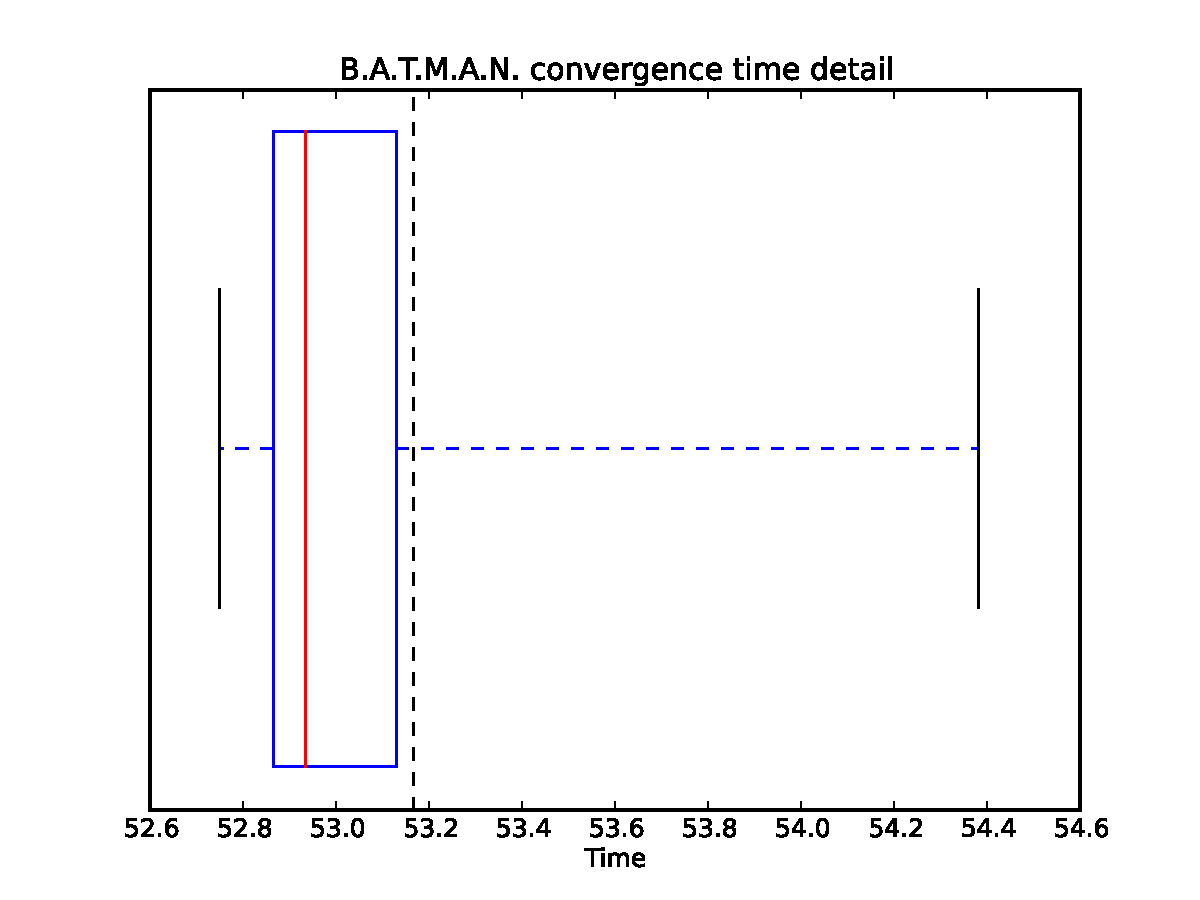
\includegraphics[width=\linewidth]{images/convergence_batman_plot_convergence_time}
    \caption{Detail of the convergence instant while using \batman\ as
             routing protocol}
    \label{pic:batman_convergence_time}
  \end{minipage}
  \hspace{0.5cm}
  \begin{minipage}[b]{0.5\linewidth}
    \centering
    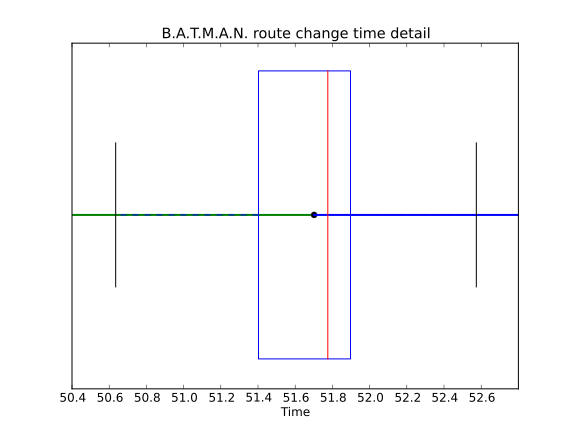
\includegraphics[width=\linewidth]{images/convergence_batman_plot_nexthop_change}
    \caption{Detail of the instant in which \batman\ changed the
                 preferred route}
    \label{pic:batman_convergence_change}
  \end{minipage}
\end{figure}


       \begin{table}[htbp]
            \centering
            \begin{tabular}{rccccccc}
            \toprule
            Kind & Average & Variance & Min & 1st Quartile &
            Median & 3rd Quartile & Max \\
            & \footnotesize{sec} & & \footnotesize{sec} & \footnotesize{sec} &
            \footnotesize{sec} & \footnotesize{sec} & \footnotesize{sec} \\
            \midrule
            Convergence & 13.166  & 0.250 & 12.749 & 12.856 & 12.935 & 13.149 &14.383\\
            Route change & 11.655 & 0.234 & 10.635 & 11.317 & 11.775 & 11.926 & 12.574\\
            \bottomrule
            \end{tabular}
            \caption{Statistics on the convergence and route change
              instants of \batman\ relative to the \emph{preferred
                route} kill time (i.e. second 40).}
            \label{tab:convergence_batman}
        \end{table}

\clearpage
\subsection{\olsr}
In this section are included the result for \olsr (see previous
subseciton for a description of the plot).
In Picture~\ref{pic:olsr_convergence} is shown the summary of our
test. A zoomed view of the convergence instant and next-hop change
instant is reported respectively in
Picture~\ref{pic:olsr_convergence_time}
and~\ref{pic:olsr_convergence_change}.


  \Picture{images/convergence_olsr_plot}
               {\textwidth}
               {Convergence plot while using \olsr\ as routing protocol}
               {pic:olsr_convergence}

\begin{figure}[bhtp]
  \begin{minipage}[b]{0.5\linewidth}
    \centering
    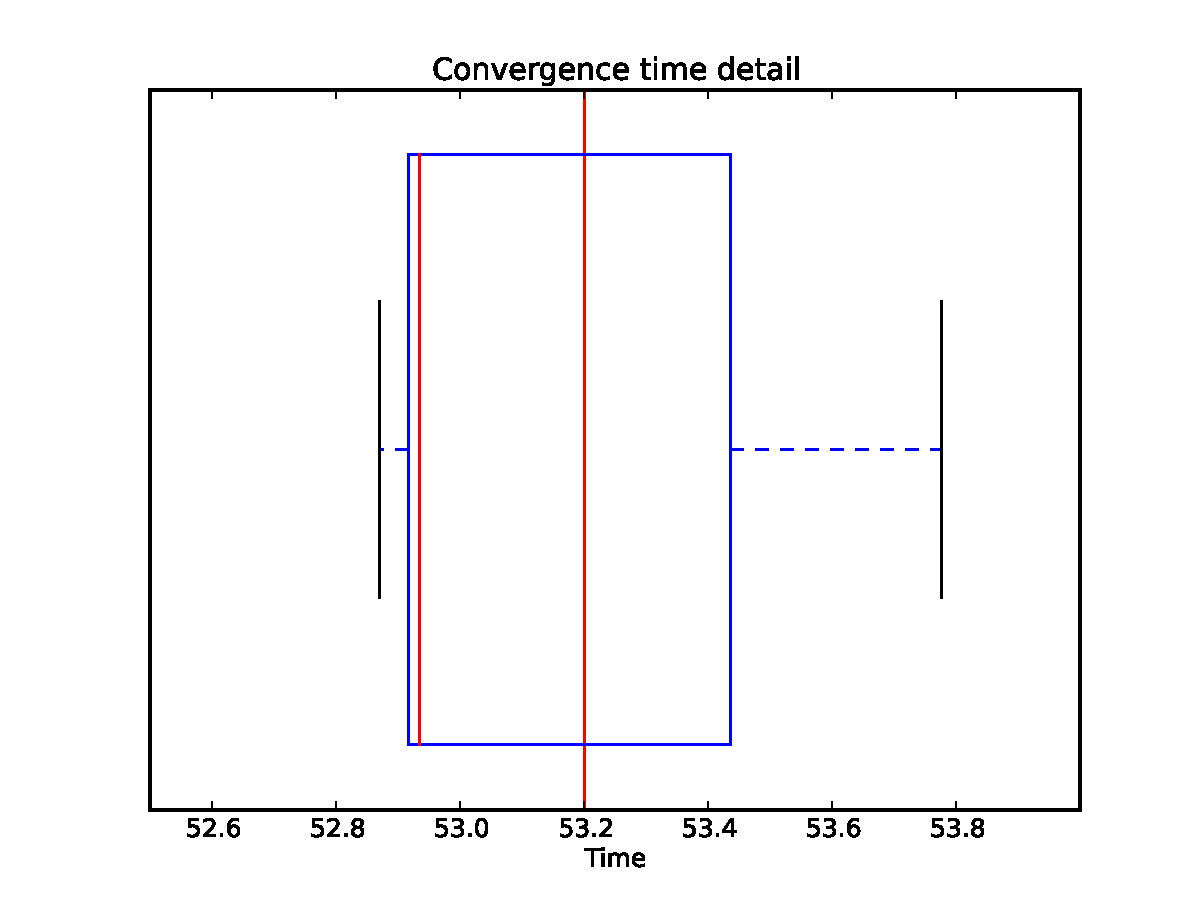
\includegraphics[width=\linewidth]{images/convergence_olsr_plot_convergence_time}
    \caption{Detail of the convergence instant while using \olsr\ as routing protocol}
    \label{pic:olsr_convergence_time}
  \end{minipage}
  \hspace{0.5cm}
  \begin{minipage}[b]{0.5\linewidth}
    \centering
    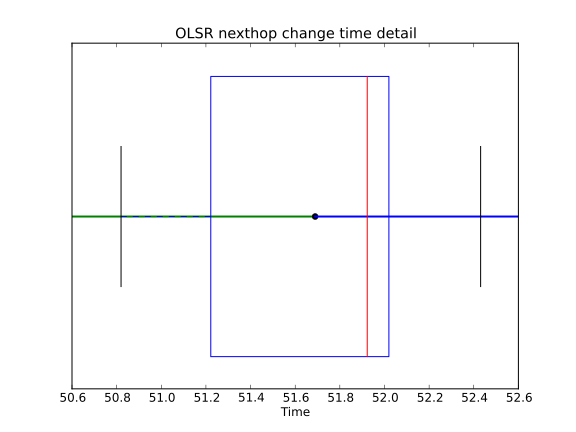
\includegraphics[width=\linewidth]{images/convergence_olsr_plot_nexthop_change}
    \caption{Detail of the instant in which \olsr\ changed the
                 preferred route}
    \label{pic:olsr_convergence_change}
  \end{minipage}
\end{figure}

       \begin{table}[htbp]
            \centering
            \begin{tabular}{rccccccc}
            \toprule
            Kind & Average & Variance & Min & 1st Quartile &
            Median & 3rd Quartile & Max \\
            & \footnotesize{sec} & & \footnotesize{sec} & \footnotesize{sec} &
            \footnotesize{sec} & \footnotesize{sec} & \footnotesize{sec} \\
            \midrule
            Convergence & 13.201 & 0.118 & 12.870 & 12.916 & 12.935 & 13.560 &13.776 \\
            Route change & 11.460 & 0.262 & 10.627 & 11.028 & 11.131 &11.827 & 12.238 \\
            \bottomrule
            \end{tabular}
            \caption{Statistics on the convergence and route change
              instants of \olsr\ relative to the \emph{preferred
                route} kill time (i.e. second 40).}
           \label{tab:convergence_olsr}
        \end{table}

\subsection{Considerations}

As can be easily seen by comparing Table~\ref{tab:convergence_batman}
with Table~\ref{tab:convergence_olsr}, the two mesh protocols
have almost equivalent performances: both show a
\emph{black out time} of about 13 seconds.

%Such a similarity in the
%results makes us think about a difference in the channel quality between
%tests, rather than an actual differences in the protocol quality.
%
%The results are so similar
%which we didn't find any important aspect which cannot be attributed
%to the mutated condition of the channel quality between tests.

An interesting aspect which we discovered about both protocols is that
they employ a mechanism to discover missing paths, which goes
beyond the simple general flow of the protocol.

This can easily be noticed by considering the behavior of \batman, which
is pretty simple to understand. The size of the sliding windows we
mentioned in Section~\ref{sec:Intro} here is relevant: the default size
value is 127 entries, and each experiment ran for 70 seconds. Each node
sends an \emph{Originator Message} per second, thus in this context:
\begin{itemize}
\item   The preference about the route only depends on how long each host
        has been working;
\item   The quality of each node keeps increasing.
\end{itemize}

The output of \batman\ in Listing~\ref{lst:batman_log} shows a time
interval in which the primary route is already down (the first row
of each block keep showing the same quality index for 10.0.0.66).
The second row of each block is about the destination (10.0.0.67) and,
despite the node is not working, the quality measure of 10.0.0.66 keeps
increasing. We would expect it dwindling to 0, while actually this
happens abruptly in the last block.

\begin{figure}[tbhp]
\begin{Verbatim}[fontsize=\footnotesize]
...
 Originator  (#/255)         Nexthop [outgoingIF]:   Potential  nexthops ... [B.A.T.M.A.N. 0.3.2 ... ]
10.0.0.66       (206)       10.0.0.66 [      eth1]:       10.0.0.66 (206)       10.0.0.68 ( 97)
10.0.0.67       (184)       10.0.0.66 [      eth1]:       10.0.0.66 (184)       10.0.0.68 (138)
10.0.0.68       (192)       10.0.0.68 [      eth1]:       10.0.0.68 (192)       10.0.0.66 (124)

  Originator  (#/255)         Nexthop [outgoingIF]:   Potential nexthops ... [B.A.T.M.A.N. 0.3.2 ... ]
10.0.0.66       (206)       10.0.0.66 [      eth1]:       10.0.0.66 (206)       10.0.0.68 ( 97)
10.0.0.67       (184)       10.0.0.66 [      eth1]:       10.0.0.66 (184)       10.0.0.68 (140)
10.0.0.68       (199)       10.0.0.68 [      eth1]:       10.0.0.68 (199)       10.0.0.66 (126)

  Originator  (#/255)         Nexthop [outgoingIF]:   Potential nexthops ... [B.A.T.M.A.N. 0.3.2 ...]
10.0.0.66       (206)       10.0.0.66 [      eth1]:       10.0.0.66 (206)       10.0.0.68 ( 97)
10.0.0.67       (185)       10.0.0.66 [      eth1]:       10.0.0.66 (185)       10.0.0.68 (144)
10.0.0.68       (202)       10.0.0.68 [      eth1]:       10.0.0.68 (202)       10.0.0.66 (126)

  Originator  (#/255)         Nexthop [outgoingIF]:   Potential nexthops ... [B.A.T.M.A.N. 0.3.2 ...]
10.0.0.66       (206)       10.0.0.66 [      eth1]:       10.0.0.66 (206)       10.0.0.68 ( 97)
10.0.0.67       (186)       10.0.0.66 [      eth1]:       10.0.0.66 (186)       10.0.0.68 (146)
10.0.0.68       (207)       10.0.0.68 [      eth1]:       10.0.0.68 (207)       10.0.0.66 (  0)

  Originator  (#/255)         Nexthop [outgoingIF]:   Potential nexthops ... [B.A.T.M.A.N. 0.3.2 ...]
10.0.0.66       (206)       10.0.0.66 [      eth1]:       10.0.0.66 (206)       10.0.0.68 ( 97)
10.0.0.67       (150)       10.0.0.68 [      eth1]:       10.0.0.66 (  0)       10.0.0.68 (150)
10.0.0.68       (211)       10.0.0.68 [      eth1]:       10.0.0.68 (211)       10.0.0.66 (  0)
...
\end{Verbatim}
\caption{Snippet of \batman\ output}
\label{lst:batman_log}
\end{figure}

This unexpected behavior implies a relevant fact: the convergence time
depends only partially on the quality of the network transmission, since
the protocol is able to detect network failures.

Even if the complexity of \olsr\ discourages us from trying to analyze in
depth its behavior, we noticed that it works similarly.
Listing~\ref{lst:olsr_log} shows, in fact, how the link to node 10.0.0.66 is
is abruptly removed from the 2-hop list for node (in the last block the
entry is no longer present), despite it's maintained with a quality
measure\footnote{A \emph{ETX} value of 1 identifies a perfect
transmission, while higher values identify worst channels} which is better
with respect to the newly chosen route.

\begin{figure}[tbhp]
\begin{Verbatim}[fontsize=\footnotesize]
...
--- 11:20:20.930522 ---------------------------------------------------- LINKS

IP address       hyst         LQ       ETX
10.0.0.68        0.000  0.482/0.576    3.596
10.0.0.66        0.000  0.729/0.765    1.793

--- 11:20:20.930547 ----------------------- TWO-HOP NEIGHBORS

IP addr (2-hop)  IP addr (1-hop)  Total cost
10.0.0.67        10.0.0.66        2.641
                 10.0.0.68        4.680
...
--- 11:20:21.030784 ---------------------------------------------------- LINKS

IP address       hyst         LQ       ETX
10.0.0.68        0.000  0.482/0.576    3.596
10.0.0.66        0.000  0.729/0.765    1.793

--- 11:20:21.030836 ----------------------- TWO-HOP NEIGHBORS

IP addr (2-hop)  IP addr (1-hop)  Total cost
10.0.0.67        10.0.0.68        4.680
...
\end{Verbatim}
\caption{Snippet of \olsr\ output}
\label{lst:olsr_log}
\end{figure}


    \end{multicols}

\clearpage
\section{Conclusions} \label{sec:Conclusions}
\vspace{-3mm}\HRule

%    \input{sections/conclusion}

\bibliographystyle{plain}

\begin{thebibliography}{99}

    \bibitem{bib:BATMAN} The \batman\ protocol:
    \url{http://www.open-mesh.org/}

    \bibitem{bib:OLSR} The \olsr\ protocol:
    \url{http://www.olsr.org/}

    \bibitem{bib:NetPerf} The \netperf\ tool (network performance
    measure)

%    \bibitem{bib:WirelessSpec} IEEE Std 802.11\texttrademark 2007, {\it
%        Part 11: Wireless LAN Medium Access Control (MAC) and Physical
%        Layer (PHY) Specifications}
%
%    % TODO: add info about artelatex and other used documents.
%
%    \bibitem{} Eric W. Weisstein,  ``Confidence Interval,'' From
%    MathWorld--A Wolfram Web Resource,
%    \url{http://mathworld.wolfram.com/ConfidenceInterval.html}

\end{thebibliography}

\end{document}
